\setchapterimage[6cm]{chapter/country/Political_Map_of_the_World_2013.png}
%\setchapterstyle{kao}
\setchapterpreamble[u]{\margintoc}
\chapter{Analysis of aspects of modern countries\protect\footnotemark}
\labch{country}

\footnotetext{\href{https://en.wikipedia.org/wiki/World_map}{Political map of the world}. 
	Author: \href{https://commons.wikimedia.org/wiki/File:Political_Map_of_the_World,_2013.png}{Central Intelligence Agency / 2015 /  Creative Commons Attribution License}.}

The chapter is devoted to the study of countries based on the knowledge base of the Wikidata international project. SPARQL queries were used in order to analyse and compare ``countries'' objects in Wikidata. A list of all currently existing countries, a list of countries ordered by date of creation, a list of demonyms of countries were generated. A bubble chart with the forms of government of countries, a graph of neighboring countries and a map of neighboring countries of Russia were constructed. In addition, conclusions were drawn regarding the completeness of the Wikidata for this topic.

%%%%%%%%%%%%%%%%%%%%%%%%%%%%%%%%%%%%%%%%%%%%%%%%%%%%%%%
\section{Instances}

Let's build a list of all countries in English and Russian (Listing \ref{lst:country}).

\begin{lstlisting}[ language=SPARQL, 
caption={List of countries in English and Russian. The result contains \num{205} countries in 2017 and \num{175} in 2020.\\\hspace{\textwidth}
SPARQL query: \href{https://w.wiki/k6L}{https://w.wiki/k6L}
},
label=lst:country]
SELECT ?country ?label_en ?label_ru
WHERE
{
	?country wdt:P31 wd:Q6256. # country
	?country rdfs:label ?label_en filter (lang(?label_en) = "en").
	?country rdfs:label ?label_ru filter (lang(?label_ru) = "ru").
}
\end{lstlisting}

According to the degree of occupancy of properties on Wikidann, one can distinguish between "full" and "empty" countries.

Examples of the most complete and developed countries on Wikidata according to ProWD are: \wdqName{Israel}{801}, \wdqName{France}{142}, \wdqName{United States of America}{30}. According to ProWD, an almost empty and uninformative country is: \wdqName{Republic of Central Lithuania}{523380}. According to ProWD, the leaders among the countries in terms of the number of properties in Wikidata are \wdqName{Israel}{801} and \wdqName{France}{142} (127 properties each), the lowest number of properties is in the \wdqName{Democratic Republic of Vietnam}{172640}  (24 properties).


%%%%%%%%%%%%%%%%%%%%%%%%%%%%%%%%%%%%%%%%%%%%%%%%%%%%%%%
\section{Age of countries}

Let's build a list of countries sorted by the date of the country's foundation (the first mention of the country) (Listing \ref{lst:age_of_country}).

\begin{lstlisting}[ language=SPARQL, 
caption={List of `instances of` ``countries sorted by inception''. The result contains \num{112} countries with completed date of foundation in 2017 and \num{199} in 2020.\\\hspace{\textwidth}
SPARQL query: \href{https://w.wiki/k6M}{https://w.wiki/k6M}
},
label=lst:age_of_country, 					
]
SELECT ?country ?countryLabel ?inception
WHERE
{
	?country wdt:P31 wd:Q6256. # country
	?country wdt:P571 ?inception. # inception
	SERVICE wikibase:label { bd:serviceParam wikibase:language "en" }
}
ORDER BY (?inception)
\end{lstlisting}

%%%%%%%%%%%%%%%% Ex 3 %%%%%%%%%%%%%%%%
\marginnote[-2.0cm]{
	\label{question:population_density}
	Identify the countries of Asia by flags and list them in ascending order of population density (fig. ~\ref{fig:flag_kor}, ~\ref{fig:flag_mongolia}, ~\ref{fig:flag_singapore}, ~\ref{fig:flag_israel}).
}

\begin{marginfigure}[-0.8cm]
	{
		\setlength{\fboxsep}{0pt}%
		\setlength{\fboxrule}{1pt}%
		\fcolorbox{gray}{gray}{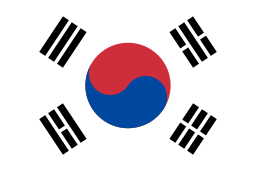
\includegraphics[width=\linewidth]{./chapter/country/256px-Flag_of_South_Korea.png}}%
	}
	\caption{First country flag.}%
	\label{fig:flag_kor}%
\end{marginfigure}

\begin{marginfigure}[3.2cm]
	{
		\setlength{\fboxsep}{0pt}%
		\setlength{\fboxrule}{1pt}%
		\fcolorbox{gray}{gray}{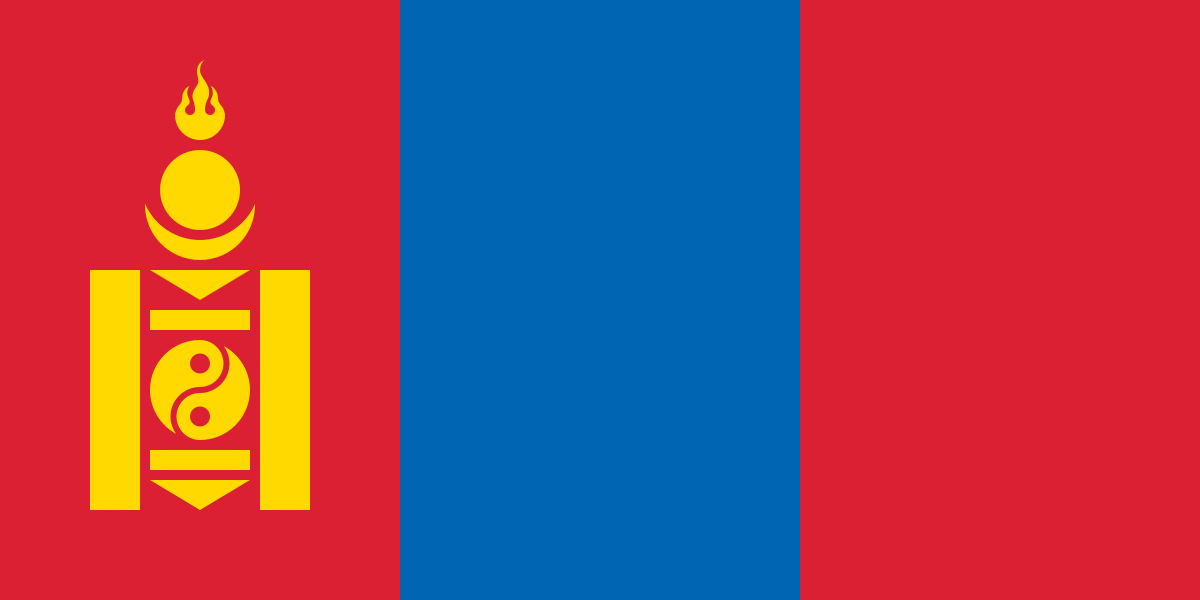
\includegraphics[width=\linewidth]{./chapter/country/256px-Flag_of_Mongolia.png}}%
	}
	\caption{Second country flag.}%
	\label{fig:flag_mongolia}%
\end{marginfigure}

As a result of the query, a list of countries with the dates of their creation was received. For example: \wdqName{Russia}{159} --- Jan 1 0862, \wdqName{Kosovo}{1246} --- Feb 17 2008, \wdqName{South Sudan}{958} --- Jul 9 2011.

According to ProWD \wdqName{France}{142} and \wdqName{Israel}{801} are the leaders in the number of objects (127 objects) among all countries. \wdqName{Land of Nod}{1929769} and \wdqName{Polska Ludowa}{11165755} have the least number of objects (3 objects).


\subsection{Countries with an unfilled inception}

Let's display a list of countries with an empty ``inception of'' property (Listing \ref{lst:without_inception}).

\begin{lstlisting}[ language=SPARQL, 
caption={List of `instances of` ``countries without a inception''. The result contains \num{100} countries without completed date of foundation in 2017 and \num{7} in 2020.\\\hspace{\textwidth}
SPARQL query: \href{https://w.wiki/k6q}{https://w.wiki/k6q}},
label=lst:without_inception
]
SELECT ?country ?countryLabel 
WHERE
{
	?country wdt:P31 wd:Q6256. # country
	MINUS { ?country wdt:P571 [] }. # inception of country is empty
	SERVICE wikibase:label { bd:serviceParam wikibase:language "en" }
}
\end{lstlisting}

\begin{marginfigure}
	{
		\setlength{\fboxsep}{0pt}%
		\setlength{\fboxrule}{1pt}%
		\fcolorbox{gray}{gray}{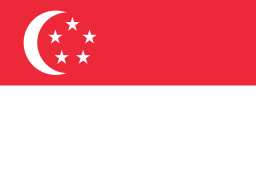
\includegraphics[width=\linewidth]{./chapter/country/256px-Flag_of_Singapore.png}}%
	}
	\caption{Third country flag.}%
	\label{fig:flag_singapore}%
\end{marginfigure}

\begin{marginfigure}
	{
		\setlength{\fboxsep}{0pt}%
		\setlength{\fboxrule}{1pt}%
		\fcolorbox{gray}{gray}{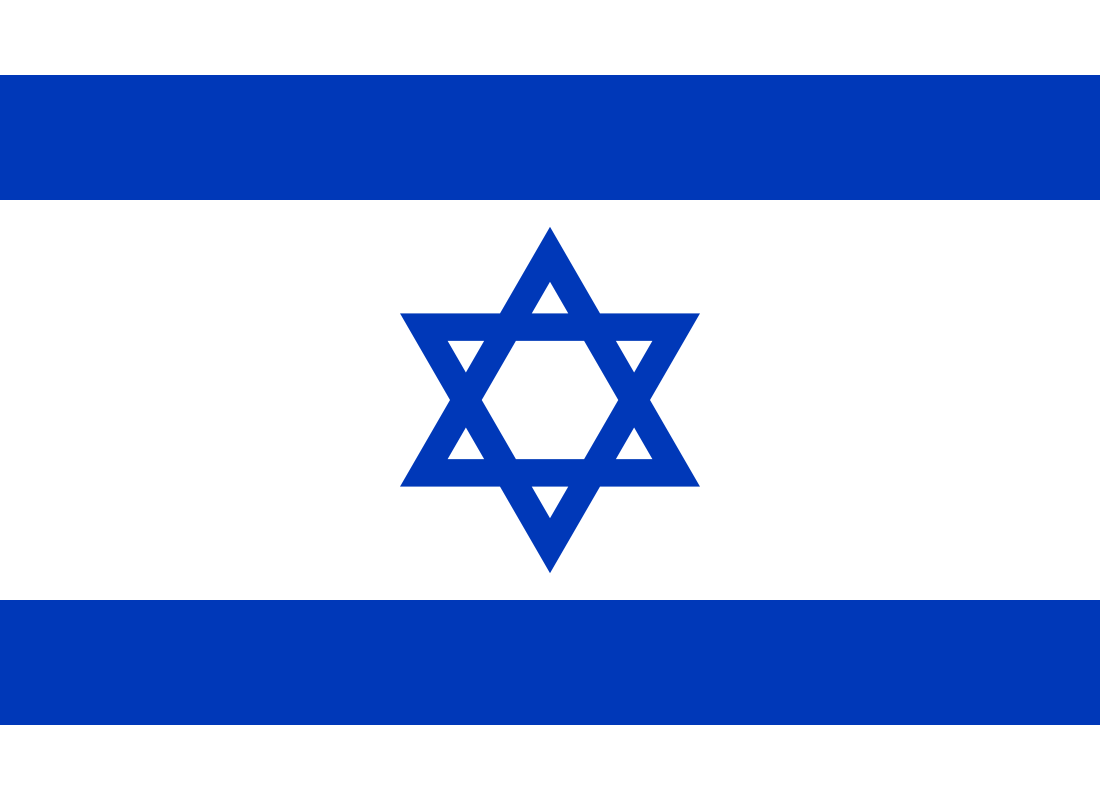
\includegraphics[width=\linewidth]{./chapter/country/256px-Flag_of_Israel.png}}%
	}
	\caption{Fourth country flag.}%
	\label{fig:flag_israel}%
\end{marginfigure}

\marginnote{
	See the answer in Exercise~\ref{answer:population_density}, page~\pageref{answer:population_density}.
}

So, on March 6 2017, the Wikidata contains 100 out of 198 entries about the currently existing countries with an unknown year of the country's foundation.

\subsection{Completeness of Wikidata}

Let's analyze the completeness of the Wikidata.

According to the ``Russian classification of countries of the world'' there are 251 countries on earth.

This task does not take into account ancient, non-existent states (for example: \wdqName{Assyria}{41137}), since they are not a ``country'' object but a ``former country'' object. Let us note that the number of former countries is an order of magnitude greater than the existing countries.

According to the category of \href{https://w.wiki/dWv}{``Alphabetical list of countries and territories''} in Russian Wikipedia, there are 252 countries.

According to the category of \href{https://en.wikipedia.org/wiki/List_of_sovereign_states}{``List of sovereign states''} in English Wikipedia, there are 206 countries.

It is not always possible to specify the exact date of the country's foundation for various reasons: absence, lack or inconsistency of written sources. For example, the basis of the Old Russian state is associated with the vocation of Varangian prince Rurik in 862, but there is no exact date (object \wdqName{Russia}{159}). Also, some modern countries were preceded by a number of others and the date of formation of which of them should be considered as the date of creation of the country is an open question (for example, \wdqName{Mongolia}{711}).


%%%%%%%%%%%%%%%%%%%%%%%%%%%%%%%%%%%%%%%%%%%%%%%%%%%%%%%
\section{List of demonyms in English}

Let's build a list of countries that have demonyms in English (Listing \ref{lst:demonym}).

\begin{lstlisting}[ language=SPARQL, 
caption={List of countries with demonyms in English. The result contains \num{197} countries with demonyms in 2017 and \num{162} in 2020.\\\hspace{\textwidth}
SPARQL query: \href{https://w.wiki/mro}{https://w.wiki/mro}},
label=lst:demonym, 
]
SELECT ?country ?countryLabel 
WHERE
{
	?country wdt:P31 wd:Q6256.       #country
	?country wdt:P1549 ?demonym.     #demonym

	FILTER((LANG(?demonym)) = "en")
	SERVICE wikibase:label { bd:serviceParam wikibase:language "en" }
}
GROUP BY ?country ?countryLabel
\end{lstlisting}


As of April 26 2017, the Wikidata contains 197 of the 202 countries with demonyms.

\subsection{List of demonyms}

Let's build a list of all demonyms in English (Listing \ref{lst:list_demonym}).

\begin{lstlisting}[ language=SPARQL, 
caption={List of demonyms in English. The result contains \num{237} demonyms in 2017 and \num{213} in 2020.\\\hspace{\textwidth}
SPARQL query: \href{https://w.wiki/mrp}{https://w.wiki/mrp}},
label=lst:list_demonym, 
]
SELECT ?country ?countryLabel ?demonym
WHERE
{
	?country wdt:P31 wd:Q6256.      #country
	?country wdt:P1549 ?demonym.    #demonym
	
	FILTER((LANG(?demonym)) = "en")
	SERVICE wikibase:label { bd:serviceParam wikibase:language "en" }
}
\end{lstlisting}

%SPARQL query (listing ~\ref{lst:list_demonym}), 237 results (2017), 213 results (2020).

On April 27 2017, the Wikidata contains 237 filled demonyms.

\subsection{Countries with unfilled demonyms}

Let's build a list of countries which do not have demonyms in English (Listing \ref{lst:without_demonym}).

\begin{lstlisting}[ language=SPARQL, 
caption={List of countries without demonyms in English. The result contains \num{5} countries without demonyms in 2017 and \num{20} in 2020.\\\hspace{\textwidth}
SPARQL query: \href{https://w.wiki/myi}{https://w.wiki/myi}},
label=lst:without_demonym, 
]
SELECT ?country ?countryLabel 
WHERE
{
	?country wdt:P31 wd:Q6256.              # country
	MINUS { ?country wdt:P1549 ?demonym.    # except demonyms
			FILTER((LANG(?demonym)) = "en") # in English
		  }    
	SERVICE wikibase:label { bd:serviceParam wikibase:language "en" }
}
GROUP BY ?country ?countryLabel
\end{lstlisting}

%SPARQL query (listing ~\ref{lst:without_demonym}), 5 results (2017), 20 results (2020).

On April 27 2017, the Wikidata comprise 5 of the 202 countries with unfilled demonyms.

\subsection{Number of demonyms in countries}

Let`s display the list of countries, ordered by the number of demonyms filled in Wikidata (Listing \ref{lst:count_demonym}).

\begin{lstlisting}[ language=SPARQL, 
caption={Count of demonyms in countries. The result contains \num{199} count of demonyms in countries in 2017 and \num{167} in 2020.\\\hspace{\textwidth}
SPARQL query: \href{https://w.wiki/mrq}{https://w.wiki/mrq}},
label=lst:count_demonym, 
]
SELECT  ?country ?countryLabel (count(*) as ?count)
WHERE
{
	?country wdt:P31 wd:Q6256.      #country
	?country wdt:P1549 ?demonym.    #demonym
	SERVICE wikibase:label { bd:serviceParam wikibase:language "en" }
}
GROUP BY ?country ?countryLabel 
ORDER BY DESC(?count)
\end{lstlisting}

%%%%%%%%%%%%%%%% Ex 4 %%%%%%%%%%%%%%%%
\marginnote{
	\label{question:official_language}
	Which of these languages are official in \href{https://en.wikipedia.org/wiki/Russia}{Russia}?
	\begin{itemize}
		\item \href{https://en.wikipedia.org/wiki/Abaza_language}{Abaza};
		\item \href{https://en.wikipedia.org/wiki/Moksha_language}{Moksha};
		\item \href{https://en.wikipedia.org/wiki/Erzya_language}{Erzya};
		\item \href{https://en.wikipedia.org/wiki/Belarusian_language}{Belarusian}.
	\end{itemize}
}
\marginnote{
	See the answer in Exercise~\ref{answer:official_languages}, page~\pageref{answer:official_languages}.
}


The United States of America Wikidata object contains the maximum number of demonyms --- 41, Great Britain --- 40, Germany --- 40, Canada --- 36 and Russia --- 34.

%%%%%%%%%%%%%%%%%%%%%%%%%%%%%%%%%%%%%%%%%%%%%%%%%%%%%%%
\section{Basic forms of government}

Let`s construct a bubble diagram of the forms of government of countries (Listing \ref{lst:form_of_government}).

\begin{lstlisting}[ language=SPARQL, 
caption={Basic form of government ranking. The result contains \num{30} basic forms of government in 2017 and \num{29} in 2020.\\\hspace{\textwidth}
SPARQL query: \href{https://w.wiki/mrr}{https://w.wiki/mrr}},
label=lst:form_of_government
]
SELECT ?bfog ?form (count(*) as ?count)
WHERE 
{
	?country wdt:P31 wd:Q6256. # country
	?country wdt:P122 ?bfog.   # subject's government
	OPTIONAL {
		?bfog rdfs:label ?form
		filter (lang(?form) = "ru")
	}
}
GROUP BY ?bfog ?form
ORDER BY DESC(?count) ASC(?form)
\end{lstlisting}

%SPARQL query (listing ~\ref{lst:form_of_government}),199 results (2017), 30 results (2017), 29 results (2020).

As a result of the query, we get a bubble chart with the most popular forms of government in countries in 2017 (fig. ~\ref{fig:bubble_chart_forms_of_government_countries_2017}) and in 2020 (fig. ~\ref{fig:bubble_chart_forms_of_government_countries_2020}).

\begin{figure}
	{
		\setlength{\fboxsep}{0pt}%
		\setlength{\fboxrule}{1pt}%
		\fcolorbox{gray}{gray}{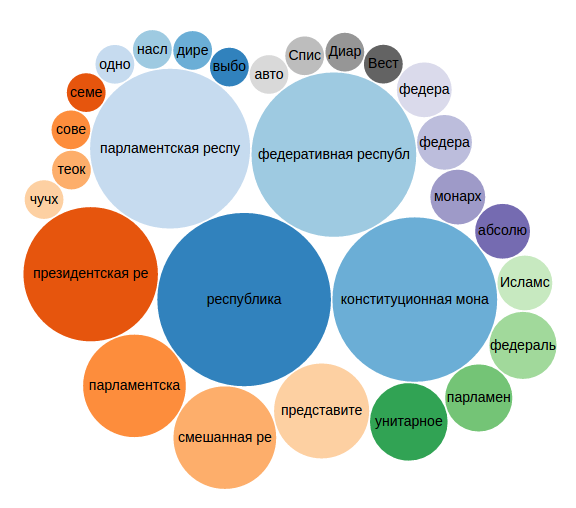
\includegraphics[width=\linewidth]{./chapter/country/Bubble_chart_forms_of_government_countries_according_to_Wikidata.png}}%
	}
	\caption{Bubble chart forms of government countries, 2017
		\\ The popular forms of government of the countries are the republic (in 20 countries), the constitutional monarchy (18), the federal republic (18), the parliamentary republic (17) and the presidential system (11) for 2017.
	}%
	\label{fig:bubble_chart_forms_of_government_countries_2017}%
\end{figure}

\begin{figure}
	{
		\setlength{\fboxsep}{0pt}%
		\setlength{\fboxrule}{1pt}%
		\fcolorbox{gray}{gray}{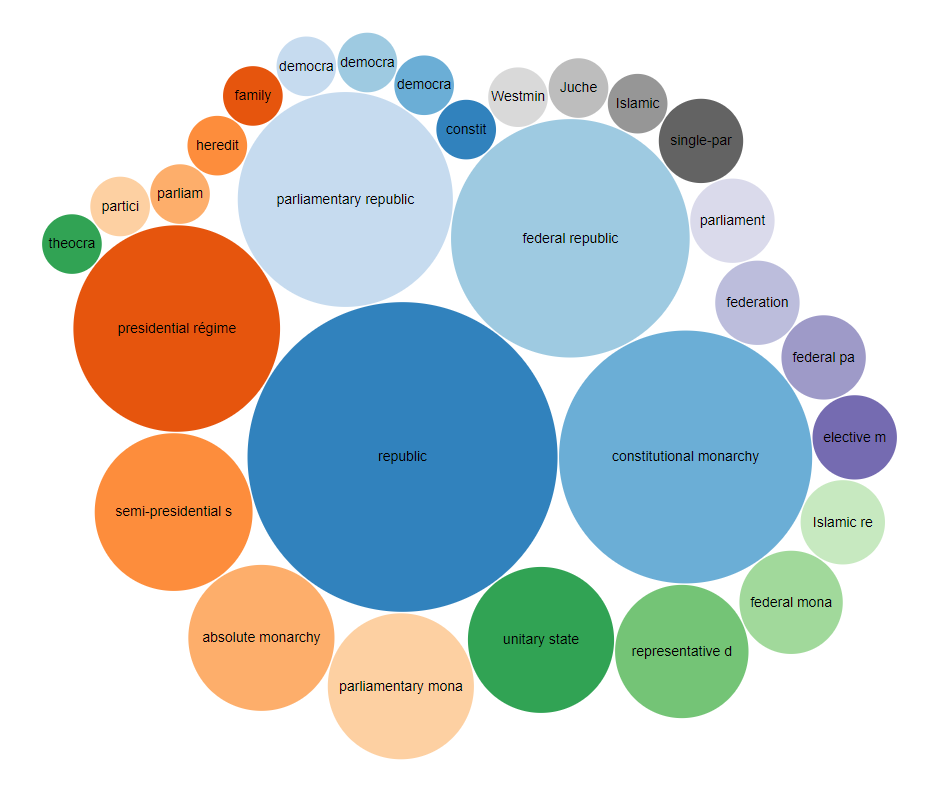
\includegraphics[width=\linewidth]{./chapter/country/Bubble_chart_forms_of_government_countries_according_to_Wikidata_2020.PNG}}%
	}
	\caption{Bubble chart forms of government countries, 2020
		\\ 
		The popular forms of government of the countries are the republic (in 27 countries), the constitutional monarchy (18), the federal republic (16), the parliamentary republic (13) and the presidential system (12) for 2020.
	}%
	\label{fig:bubble_chart_forms_of_government_countries_2020}%
\end{figure}

%%%%%%%%%%%%%%%%%%%%%%%%%%%%%%%%%%%%%%%%%%%%%%%%%%%%%%%
\section{Neighboring countries}

We will construct a graph of neighboring countries (Listing \ref{lst:neighboring_countries}).

\begin{lstlisting}[ language=SPARQL, 
caption={Neighboring countries graph. The result contains \num{795} neighboring countries in 2017 and \num{698} in 2020.\\\hspace{\textwidth}
SPARQL query: \href{https://w.wiki/mrs}{https://w.wiki/mrs}},
label=lst:neighboring_countries
]
#Neighboring countries graph
#defaultView:Graph
SELECT ?country ?countryLabel ?sharesBorderWith 
?sharesBorderWithLabel
WHERE
{
	?country wdt:P31 wd:Q6256.
	
	SERVICE wikibase:label { bd:serviceParam wikibase:language "en" }
	OPTIONAL { ?country wdt:P47 ?sharesBorderWith. }
}
\end{lstlisting}

%SPARQL query (listing ~\ref{lst:neighboring_countries}), 795 results (2017), 698 results (2020).

\begin{figure*}
	{
		\setlength{\fboxsep}{0pt}%
		\setlength{\fboxrule}{1pt}%
		\fcolorbox{gray}{gray}{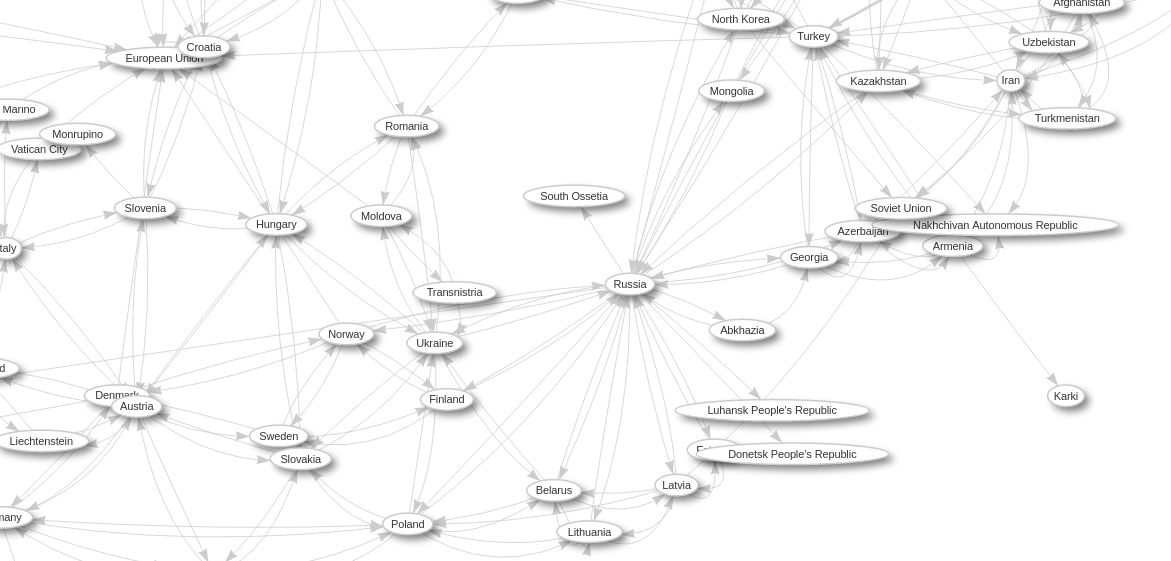
\includegraphics[width=\linewidth]{./chapter/country/Neighboring_countries_graph_according_to_Wikidata.png}}%
	}
	\caption{Neighboring countries graph, 2017.
	}%
	\label{fig:neighboring_countries_2017}%
\end{figure*}

\begin{figure*}
	{
		\setlength{\fboxsep}{0pt}%
		\setlength{\fboxrule}{1pt}%
		\fcolorbox{gray}{gray}{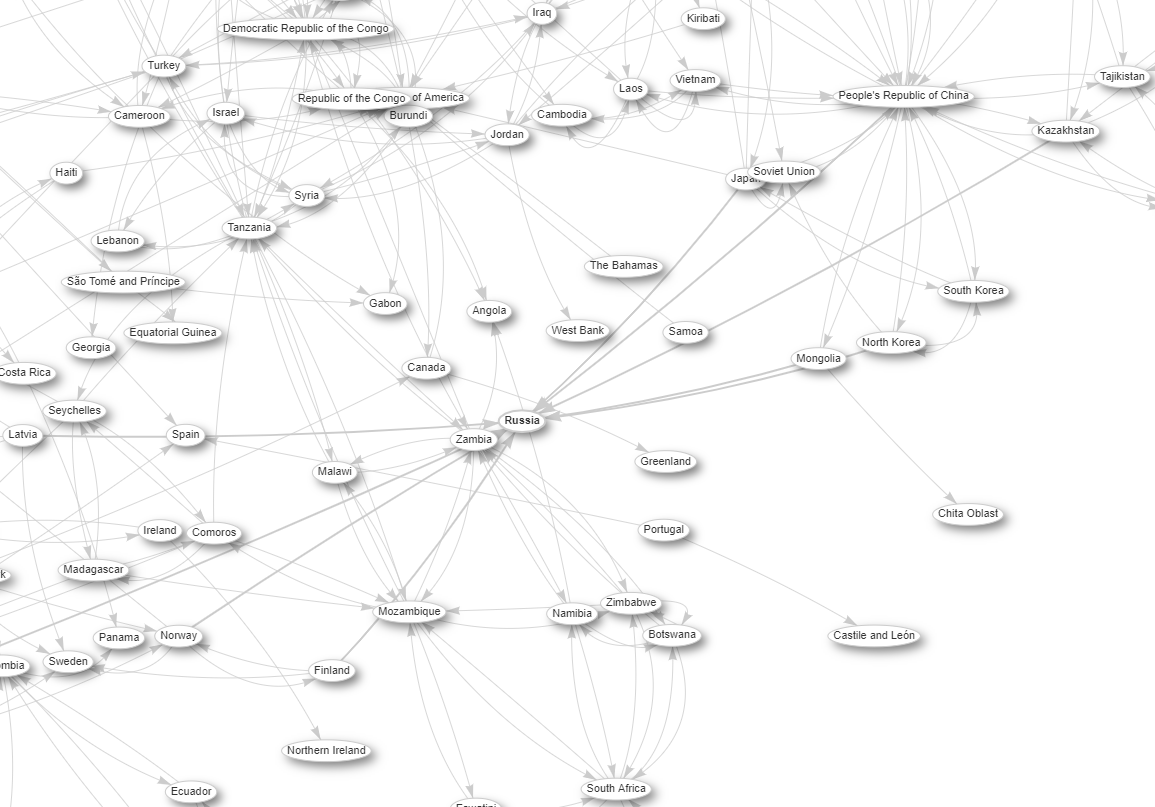
\includegraphics[width=\linewidth]{./chapter/country/Neighboring_countries_graph_in_russian_according_to_Wikidata_2020_en_upload.png}}%
	}
	\caption{Neighboring countries graph, 2020.
	}%
	\label{fig:neighboring_countries_2020}%
\end{figure*}

As a result of the query, we get a graph with 787 edges on 2017 (fig. ~\ref{fig:neighboring_countries_2017}) and 698 edges on 2020 (fig. ~\ref{fig:neighboring_countries_2020}), where the edge is a neighborhood between the two countries. The graph represents several connected components, since there are island countries that do not have neighbors (for example, Mauritius, Maldives, Madagascar).

\subsection{Neighboring countries of Russia}

We will construct a graph of neighboring countries of Russia (Listing \ref{lst:neighboring_countries_ru}).

\begin{lstlisting}[ language=SPARQL, 
caption={Map of neighboring countries of Russia. The result contains \num{22} neighboring countries in 2020.\\\hspace{\textwidth}
SPARQL query: \href{https://w.wiki/rMR}{https://w.wiki/rMR}},
label=lst:neighboring_countries_ru
]
# Map of neighboring countries of Russia
#defaultView:Map
SELECT ?border_country ?border_countryLabel ?coords ?layer
WHERE 
{
	?border_country wdt:P47 wd:Q159.  # country has border with Russia
	OPTIONAL { ?border_country wdt:P3896 ?coords. }
	BIND ( ?coords AS ?layer )
	SERVICE wikibase:label { bd:serviceParam wikibase:language "en". }
}
\end{lstlisting}

As a result of executing the query, we get a map of neighboring countries of Russia (Fig. ~\ref {fig: neighboring_countries_ru}), which includes the following countries:
\begin{enumerate}
	\item \wdqName{Japan} {17}
	\item \wdqName{Norway} {20}
	\item \wdqName{Finland} {33}
	\item \wdqName{Poland} {36}
	\item \wdqName{Lithuania} {37}
	\item \wdqName{People's Republic of China} {148}
	\item \wdqName{Belarus} {184}
	\item \wdqName{Estonia} {191}
	\item \wdqName{Latvia} {211}
	\item \wdqName{Ukraine} {212}
	\item \wdqName{Azerbaijan} {227}
	\item \wdqName{Georgia} {230}
	\item \wdqName{Kazakhstan} {232}
	\item \wdqName{DPRK} {423}
	\item \wdqName{European Union} {458}
	\item \wdqName{Mongolia} {711}
	\item \wdqName{Hokkaido} {35581}
	\item \wdqName{Racha-Lechkhumi and Kvemo-Svaneti} {38893}
	\item \wdqName{Chechen Republic of Ichkeria} {210036}
	\item \wdqName{Donetsk People's Republic} {16150196}
	\item \wdqName{Luhansk People's Republic} {16746854}
	\item \wdqName{Republic of Abkhazia} {31354462}
\end{enumerate}


\begin{figure}
	{
		\setlength{\fboxsep}{0pt}%
		\setlength{\fboxrule}{1pt}%
		\fcolorbox{gray}{gray}{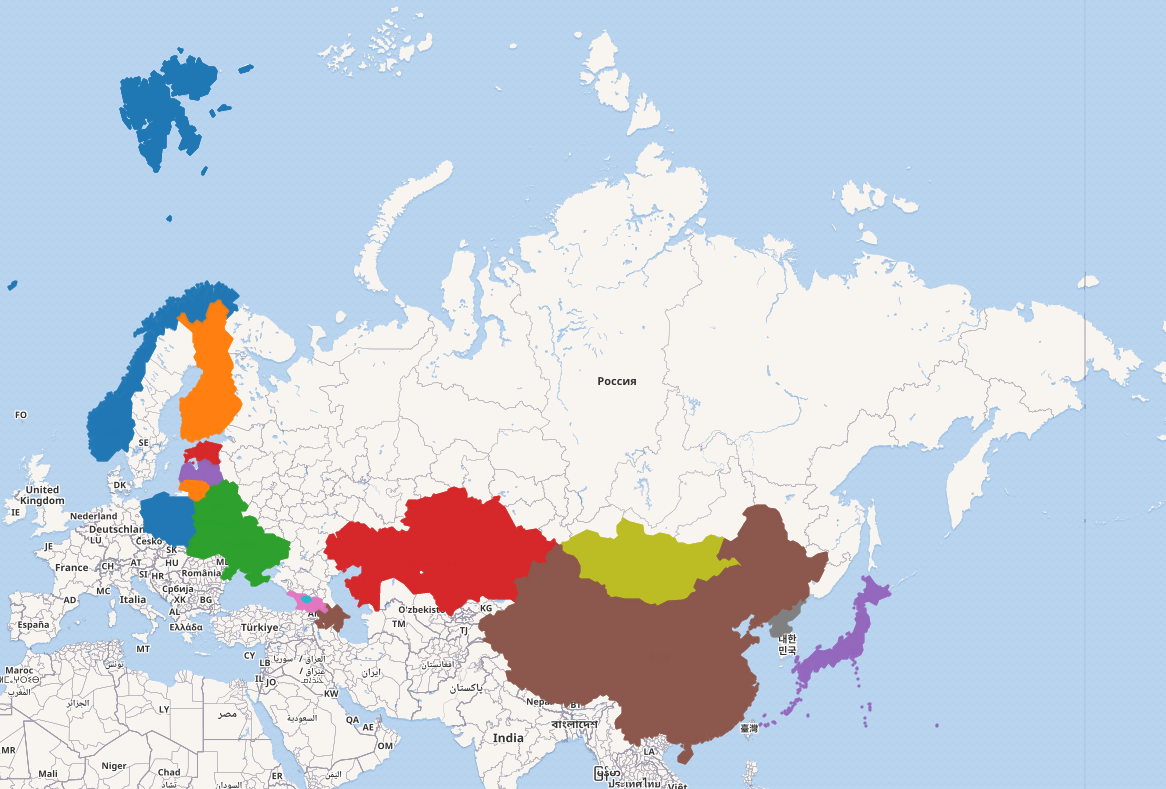
\includegraphics[width=\linewidth]{./chapter/country/Map_of_neighboring_countries_of_Russia_en.png}}%
	}
	\caption{Map of neighboring countries of Russia, 2020.
	}%
	\label{fig:neighboring_countries_ru}%
\end{figure}
%%%%%%%%%%%%%%%%%%%%%%%%%%%%%%%%%%%%%%%%%%%%%%%%%%%%%%%
\section{Exercises}
\begin{enumerate}
	\item For each country display its flag and motto.
	\item Draw a map with the marked capitals of all the existing countries.
	\item Calculate the first five countries with the largest population density for each continent.
	\item Construct a column diagram showing the distribution of the number of countries by form of government. Estimate whether this distribution has a heavy tail.
	\item Build a list the countries ordered by the number of neighbors. Which countries have the maximum and minimum number of neighbors, what is the average number of neighbors? Is there a correlation between this parameter and some other parameter of the countries?
\end{enumerate}